\chapter{Zadatak 3}

U ovom zadatku je potrebno relejnom metodom podesiti parametre PID regulatora tako da ostvarimo faznu marginu od $60^{\circ}$. Prenosna funkcija sistema je:
	\[G(s)=\frac{4}{256s^5+448s^4+304s^3+100s^2+16s+1} \]

Korišten je relej sa histerezisom od $\epsilon=0.1$ i amplitudom izlaznog signala d=1. Shema simulink modela koji omogućava ovo podešavanje je data na slici (slika \ref{fig:z3_1}).

\begin{figure} [H]
  \centering
  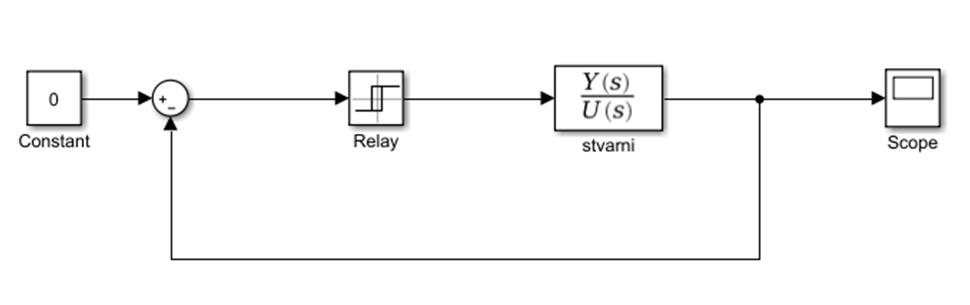
\includegraphics[width=0.8\textwidth]{z3_1}
  \caption{Simulink model pomoću kojeg je određena amplituda i kružna učestanost oscilacija na izlazu sistema}
  \label{fig:z3_1}
\end{figure}
 
Nakon izvršene simulacije izmjerena je amplituda i kružna učestanost oscilacija na izlazu sistema (slika \ref{fig:z3_2}). Dobivene su vrijednosti amplitude A=1.66 i perioda $T_0=27s$, odakle se dobije kružna učestanost $\omega_0=2\pi/T_0 =0.2327 rad/s$.

\begin{figure} [H]
  \centering
  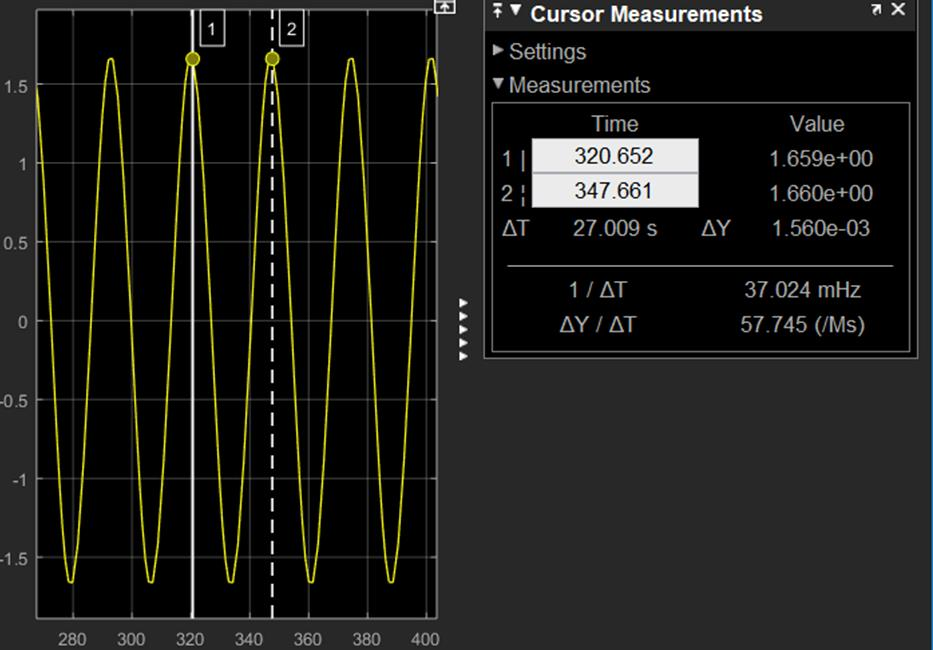
\includegraphics[width=0.8\textwidth]{z3_2}
  \caption{Mjerenje amplitude i kružne učestanosti nastalih stabilnih oscilacija}
  \label{fig:z3_2}
\end{figure}

Na osnovu naredne tabele podešavamo naš PID regulator (slika \ref{fig:z3_3}).

\begin{figure} [H]
  \centering
  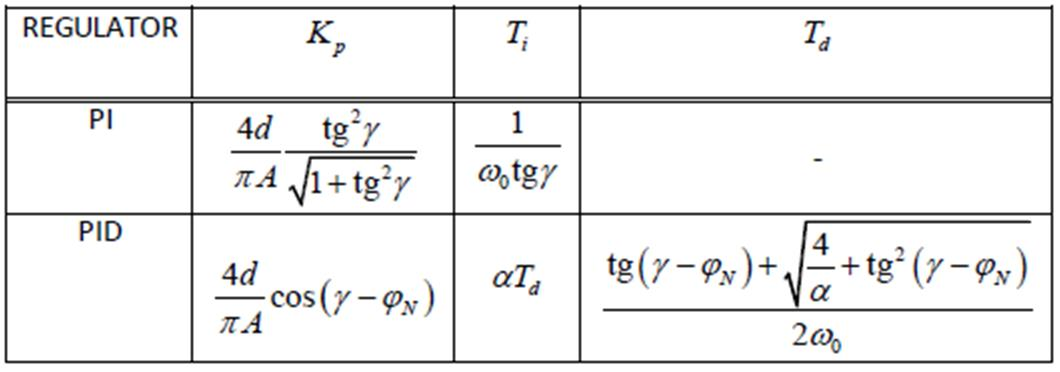
\includegraphics[width=0.5\textwidth]{z3_3}
  \caption{Tabela podešavanja regulatora relejnom metodom}
  \label{fig:z3_3}
\end{figure}

Već su prethodno date ili izmjerene vrijednosti: A=1.66, $\omega_0=0.2327$, d=1, $\epsilon=0.1$. Zahtjev na faznu marginu je $\gamma=60^{\circ}$.

Preostale vrijednosti koje je potrebno izračunati da bi mogli odrediti parametre PID regulatora su:
	\[\phi_n=atan\frac{\epsilon}{\sqrt{A^2-\epsilon^2}}=3.4536^{\circ}\]

Sada možemo odrediti parametre PID regulatora prema tabeli (slika \ref{fig:z3_3}). Dobijamo:        $K_p=0.4228, T_i=28.5979 i T_d=7.1495$. Dobija se ukupna prenosna funkcija PID regulatora:
	\[G_{PID} (s)=\frac{86.45s^2+12.09s+0.4228}{28.6s}\]

Ukupna prenosna funkcija otvorenog sistema je:
	\[G_o (s)=G_{PID} (s)G(s)=\frac{345.8s^2+48.37s+1.691}{7321s^6+12810s^5+8694s^4+2860s^3+457.6s^2+28.6s} \]

Bode dijagrame za provjeru fazne margine crtamo na osnovu ukupne prenosne funkcije otvorenog sistema $G_o (s)$. Možemo očitati da je dobivena fazna margina od $59^{\circ}$ (slika \ref{fig:z3_4}), što je zadovoljavajuće s obzirom na zahtjev na faznu marginu od $\gamma=60^{\circ}$.

\begin{figure} [H]
  \centering
  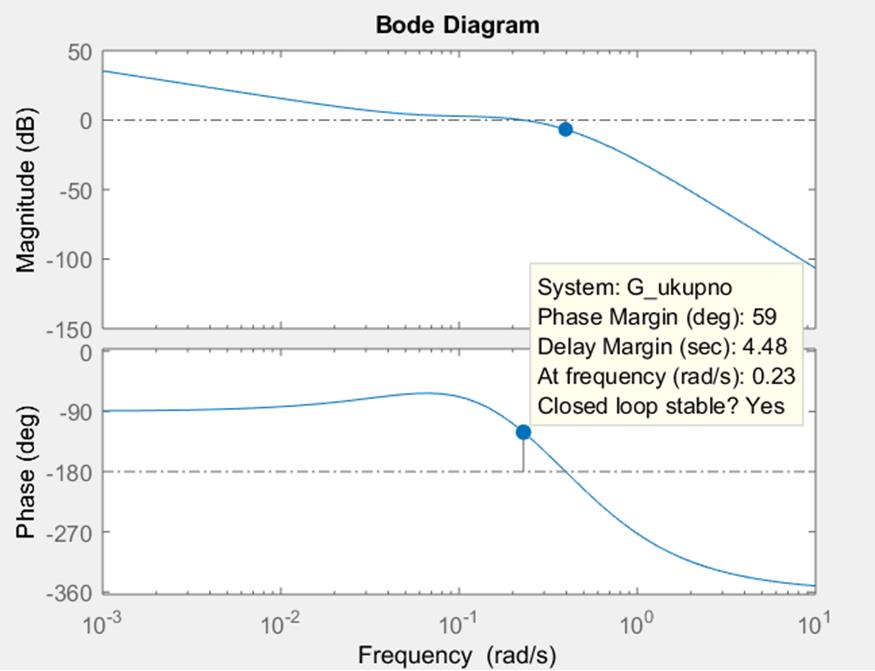
\includegraphics[width=0.8\textwidth]{z3_4}
  \caption{Bode dijagram sistema sa PID regulatorom u otvorenom ($G_o (s)$)}
  \label{fig:z3_4}
\end{figure}




























